\chapter{Evaluation on the held-out test set} \label{ch:heldout}

Up to now, we have performed all evaluation on our development set. In this
chapter, we will evaluate our best models on the held-out test set we created
in section \ref{sec:datasplit} in order to get our final estimate on our
models' performance on unseen data. Since we have used results on the
development set to inform decisions about model selection and tuning of
hyperparameters, we have arguably trained these properties on the development
set. Moreover, even if the development set has not been used by the gradient
descent methods to tune the weights of a neural network, we have monitored
our metrics on the development set and used them to stop training at a point
where the performance on validation data is most favourable.

While the results on the development set are informative, the final
evaluation on the test set is even more so, since the test data has not been
used at all for training models, and thus is our best proxy for real-world
data outside of our dataset.

In the development set, the size of peripheral classes is very small. Only
one document has label `A2', and only three have the label `C1'. This has
influenced our macro \FI scores quite a bit, since the \FI score for the `A2'
class has always been either 0 or 1. The distribution of classes in the test
set is such that the smallest class, `A2', is supported by three documents.
We therefore expect the macro \FI scores in this evaluation to be different.
It is however not as hard to compare micro \FI scores, as they are not
influenced by the support of the classes.

In the linear models, we have not previously used the development set as
validation data. Therefore, when we evaluate on the test set, we have merged
the training and development set to use as training data. This also means
that the input features are not exactly the same, since the features are
decided by the training data.

For the neural models, however, we train exactly like before. The training
set is used for gradient descent, while we monitor the macro \FI score on the
development set and remember the epoch that had the highest \FI score, so
that we can restore the network weights from this epoch at the end of
training.

\begin{table}
  \centering
  \begin{tabular}{lrrrr}
    \toprule
             & \multicolumn{2}{c}{All labels} & \multicolumn{2}{c}{Collapsed labels} \\
    \cmidrule(lr){2-3}
    \cmidrule(lr){4-5}
    Model      & Macro \FI & Micro \FI & Macro \FI & Micro \FI \\
    \midrule
    Majority   &  $0.045$  &  $0.187$  &  $0.127$  &  $0.341$ \\
    \midrule
    % $BEGIN autotable final_test_eval
    % $META models-per-row=2 columns-per-model=macrof1,microf1
    % $ROW SVR BOW: linear_svr-04-24_13-29-06  linear_svr-04-24_13-30-41
    % $ROW SVR POS: linear_svr-04-24_13-30-09  linear_svr-04-24_13-31-01
    % \midrule
    % $ROW RNN1: rnn-26805083_0_model_test_eval rnn-26805084_0_model_test_eval
    % $ROW RNN2: rnn-26805083_1_model_test_eval rnn-26805084_1_model_test_eval
    % $ROW RNN1 Multi: rnn-multi-26805083_2_model_test_eval rnn-multi-26805084_2_model_test_eval
    % $ROW RNN2 Multi: rnn-multi-26805083_3_model_test_eval rnn-multi-26805084_3_model_test_eval
    % $END autotable
    SVR BOW & $0.231$ & $0.285$ & $0.420$ & $0.602$ \\
    SVR POS & $0.271$ & $0.350$ & $0.422$ & $0.602$ \\
    \midrule
    RNN1 & $0.291$ & $0.439$ & $0.478$ & $\mathbf{0.724}$ \\
    RNN2 & $\mathbf{0.388}$ & $\mathbf{0.480}$ & $\mathbf{0.511}$ & $\mathbf{0.724}$ \\
    RNN1 Multi & $0.266$ & $0.398$ & $0.509$ & $0.707$ \\
    RNN2 Multi & $0.356$ & $0.447$ & $0.443$ & $\mathbf{0.724}$ \\
    \bottomrule
  \end{tabular}
  \caption[Evaluation results on the held-out test set]{
      Results from evaluating on the held-out test set. SVR is support vector
      regression. Hyperparameters for RNN1 and RNN2 are found in table
      \ref{tab:rnn-parameters}. Multi-task models use an auxiliary task
      weight of $0.1$.
  }
  \label{tab:held-out-results}
\end{table}

The linear models have lower scores on the evaluation metrics when evaluated
on the test set than they did previously. SVR BOW and SVR POS had macro \FI
scores of $0.444$ and $0.334$, respectively, on the development set. On the
test set, the respective scores are $0.231$ and $0.271$. We still see that
\ac{RNN} models produce higher scores.

The best macro \FI score on the test set is $0.388$, noticeably less than the
highest macro \FI score we saw when we evaluated on the development set,
which was $0.460$ using the RNN1 system. However, the micro \FI scores are
comparable. The highest micro \FI score among all the RNN models we trained
in single-task mode in chapter \ref{ch:sequencemodels} was $0.463$. The RNN2
model has the highest micro \FI score on the test set, as seen in table
\ref{tab:held-out-results}. This model had a micro \FI of $0.447$ when
evaluated on the development set, which increased to $0.480$ when evaluating
on the test set.

We assume that the differences in macro \FI we observe when evaluating on
different splits are mostly caused by the different distribution of labels in
the development and test sets, and are not indicative of poor generalization.
The micro \FI scores are similar on both splits, which supports our
assumption. If the models turned out to not generalize beyond the development
set, we would expect performance to drop on both metrics, not only on the
macro \FI score.


\section{Multi-task predictions}

We examine the confusion matrices for our best multi-task model, `RNN2 Multi',
on the test set. The plot is given in figure \ref{fig:multi-test-cm}.

\begin{figure}
  \centering
  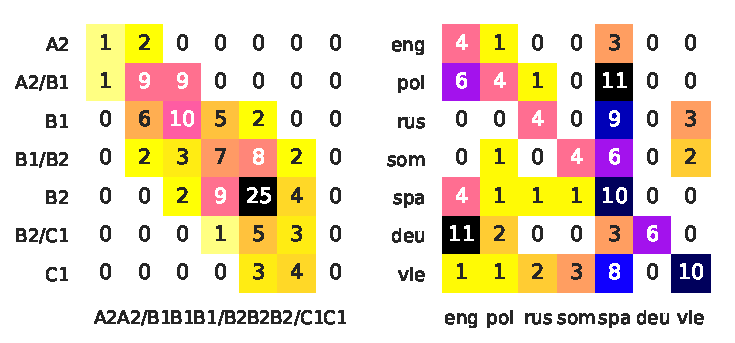
\includegraphics{multi-test-cm}
  
  \caption[Multi-task confusion matrices]{
    Confusion matrices for RNN2 Multi on the held-out test set. \ac{AES} task
    on the left, \ac{NLI} task on the right. The numbers are counts.
  }
  \label{fig:multi-test-cm}
\end{figure}

The confusion matrix on CEFR scores looks a lot like previous confusion matrices
for the task. Predictions follow a blurry diagonal.

In the confusion matrix for \acp{L1}, we see that all languages are predicted
to be Spanish at some point. German is predicted with 100\% precision,
however a lot of German texts are wrongly classified as English. This seems
reasonable since English and German are similar languages in the same
language family. However, the Slavic languages are not confused for each
other, as one might expect, but rather Russian and Polish are both commonly
mistaken for Spanish.


\section{Predictions on the control corpus}

As a sanity check, we also use our model to automatically assign CEFR labels
to the texts in ASK's control corpus, which consists of texts written by
native Norwegian speakers. These texts are written under similar conditions as
the essays in the main corpus, at least with respect to essay prompts and time
limits. However, the authors in the control corpus have not actually taken the
test in order to prove their proficiency in their native language, unlike the
authors in the main corpus, who have had a stake in their test results.

There is no canonical CEFR score associated with
these texts in the corpus, but we assume that native Norwegian speakers would
generally be rated at a high level of proficiency in the CEFR framework.

\begin{figure}
  \centering
  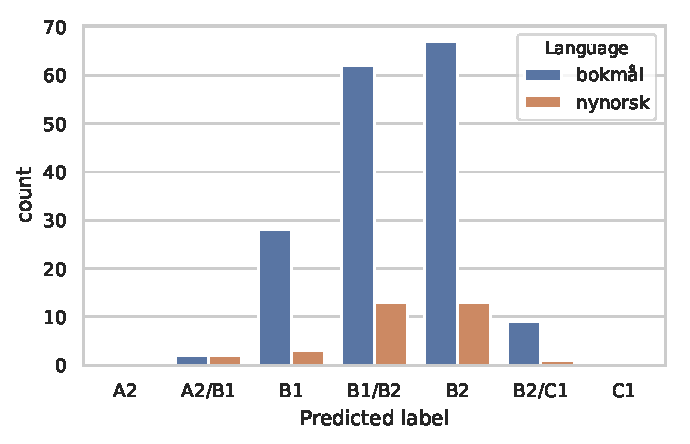
\includegraphics{native-predictions}
  \caption[Predicted CEFR score for native Norwegian speakers]{
    Counts of predicted labels for texts in the ASK control corpus, written by
    native speakers of Norwegian. `Nynorsk' and `bokmål' are the two official
    written variants of Norwegian.
  }
  \label{native-predictions}
\end{figure}

We chose the single-task RNN2 model to perform the predictions and plotted the
distribution of predictions in figure \ref{native-predictions}. The model predicts
very few texts from the control corpus to have a proficiency of more than B2,
which seems unlikely.
